\section{Operating System Basics}
\subsection{Introduction}

\begin{frame}[fragile]{Abstraction of CPU}

	Take a closer look at the CPU die:

	\only<1>{
		\begin{figure}[H]
			\centering
			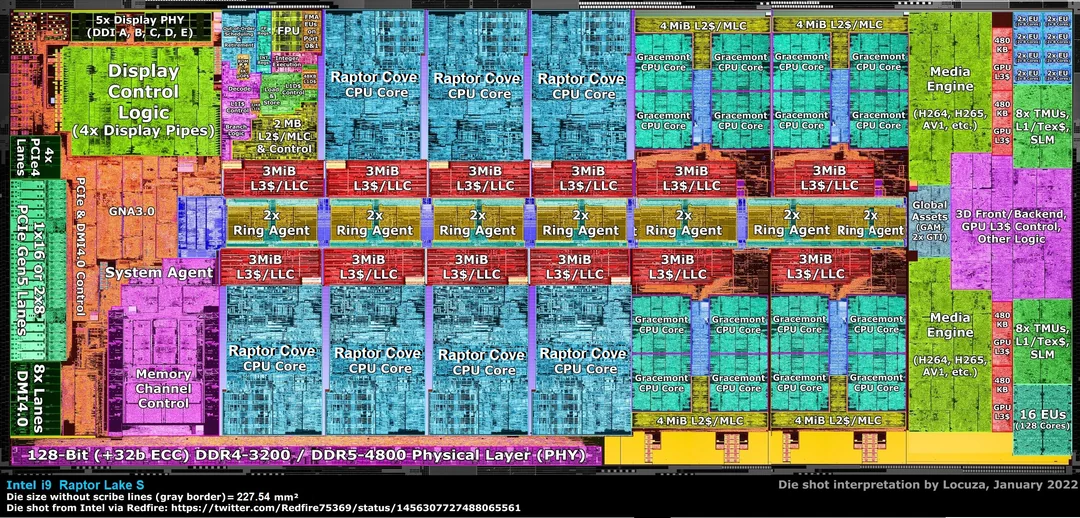
\includegraphics[width=0.75\textwidth]{day3/img/cpu-die.png}
			\caption{Intel Core i9 13900K Die Shot}
		\end{figure}
	}

	\only<2->{
		\begin{columns}
			\begin{column}{0.6\textwidth}
				\begin{figure}[H]
					\centering
					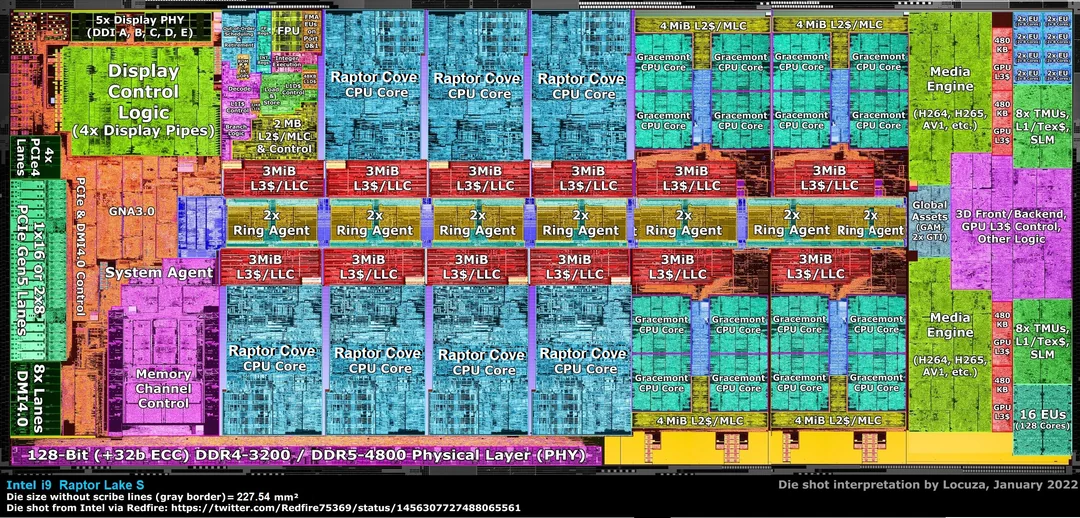
\includegraphics[width=\textwidth]{day3/img/cpu-die.png}
				\end{figure}
			\end{column}
			\begin{column}{0.4\textwidth}
				\begin{figure}[H]
					\centering
					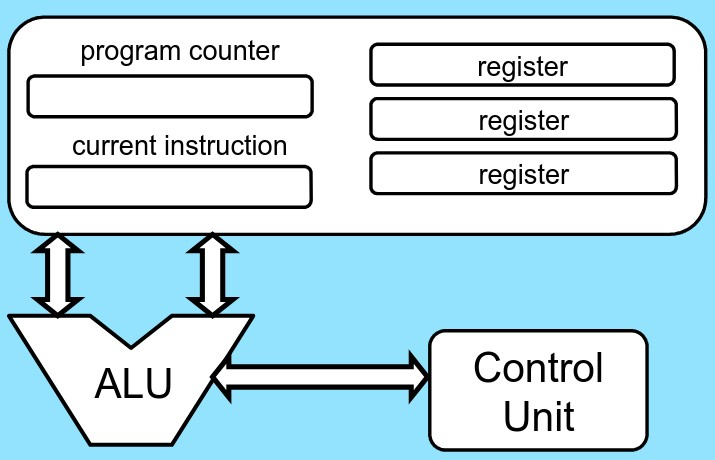
\includegraphics[width=\textwidth]{day3/img/cpu-abstract.jpg}
				\end{figure}
			\end{column}
		\end{columns}

		\begin{itemize}
			\item<3-> \textbf{Program Counter}
			\item<4> Register: stores data processed by the CPU (\textbf{a.k.a. context})
		\end{itemize}

	}

\end{frame}

\begin{frame}[fragile]{Memory Hierarchy}
	\only<1>{
		\begin{figure}[H]
			\centering
			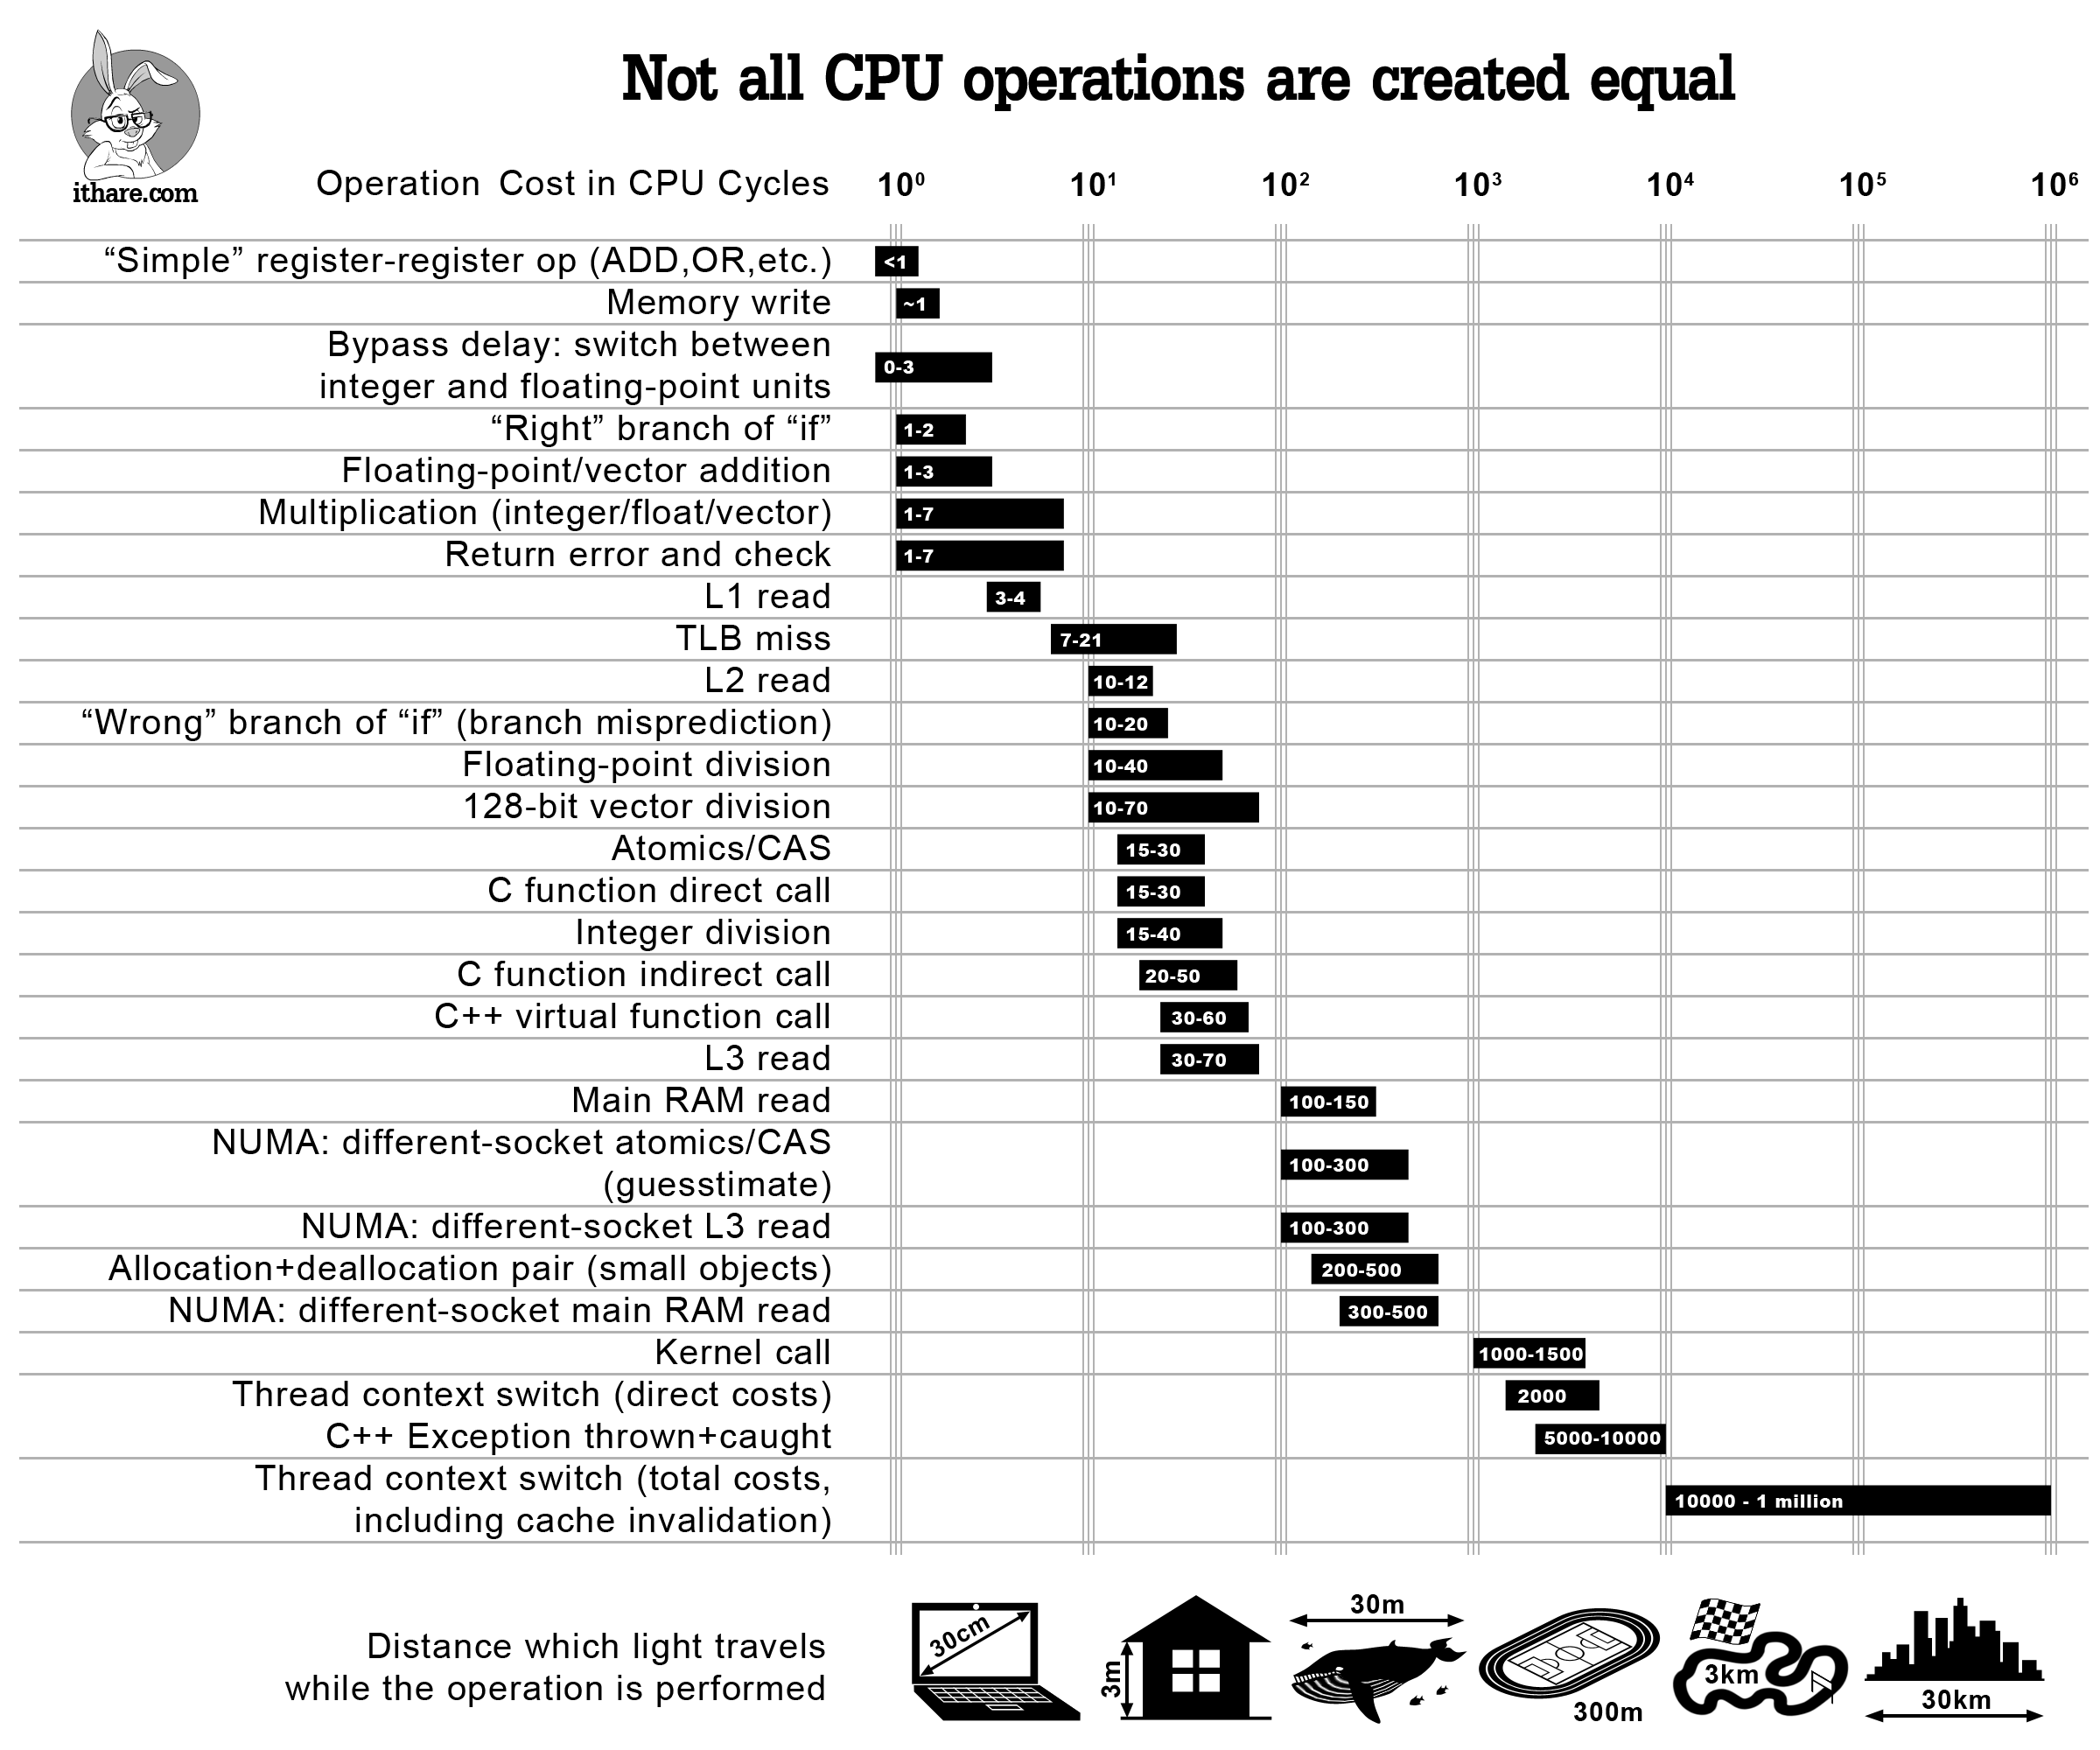
\includegraphics[width=0.55\textwidth]{day3/img/latency-2.png}
		\end{figure}
	}
	\only<2>{
		\begin{figure}[H]
			\centering
			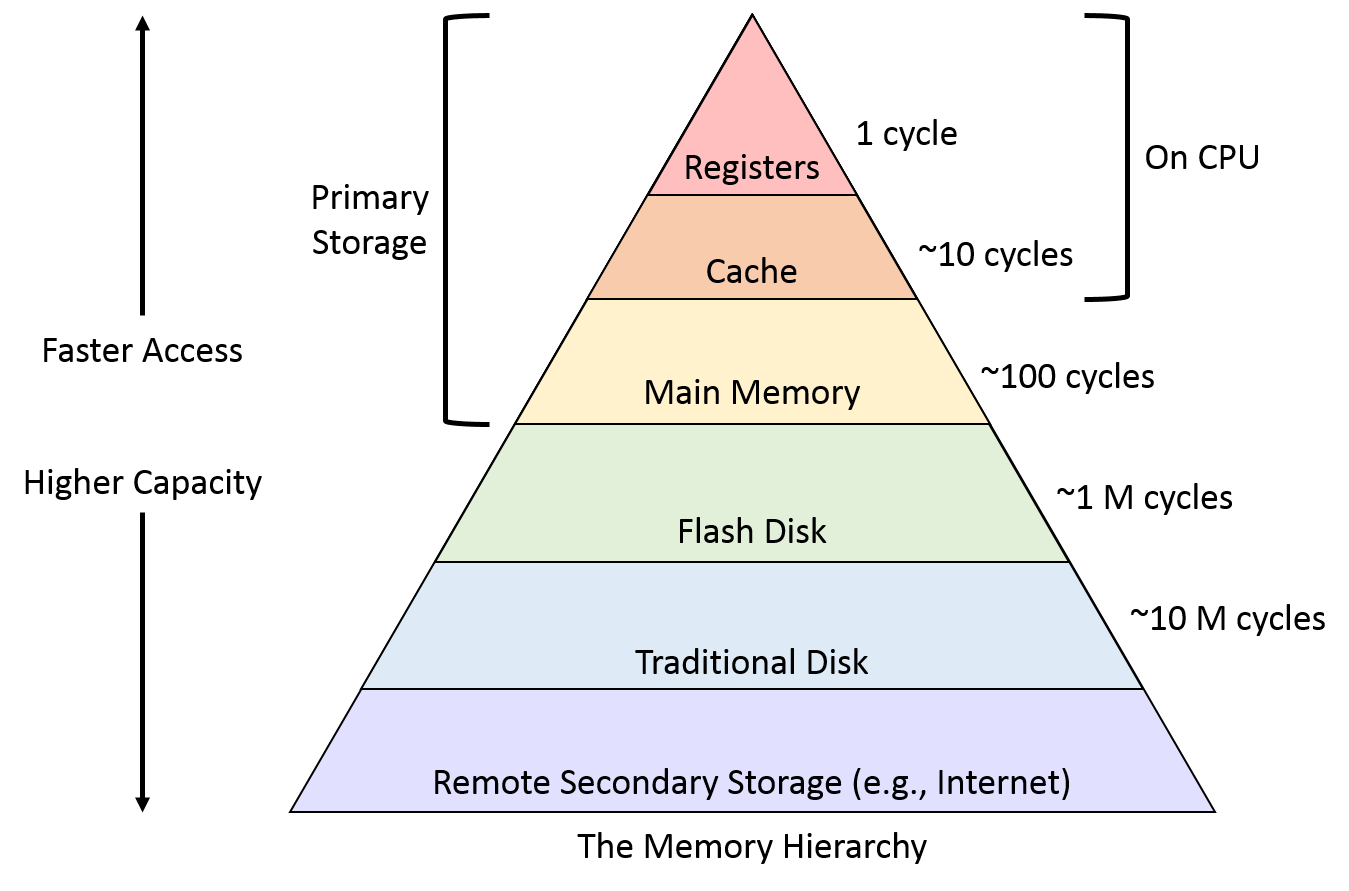
\includegraphics[width=0.7\textwidth]{day3/img/mem-hi.png}
		\end{figure}
	}
\end{frame}

\begin{frame}[fragile]{\emoji{thinking} What is an Operating System?}
	Common operating systems we see in 2025:
	\begin{columns}[T]
		\begin{column}{0.6\textwidth}
			\begin{figure}[H]
				\centering
				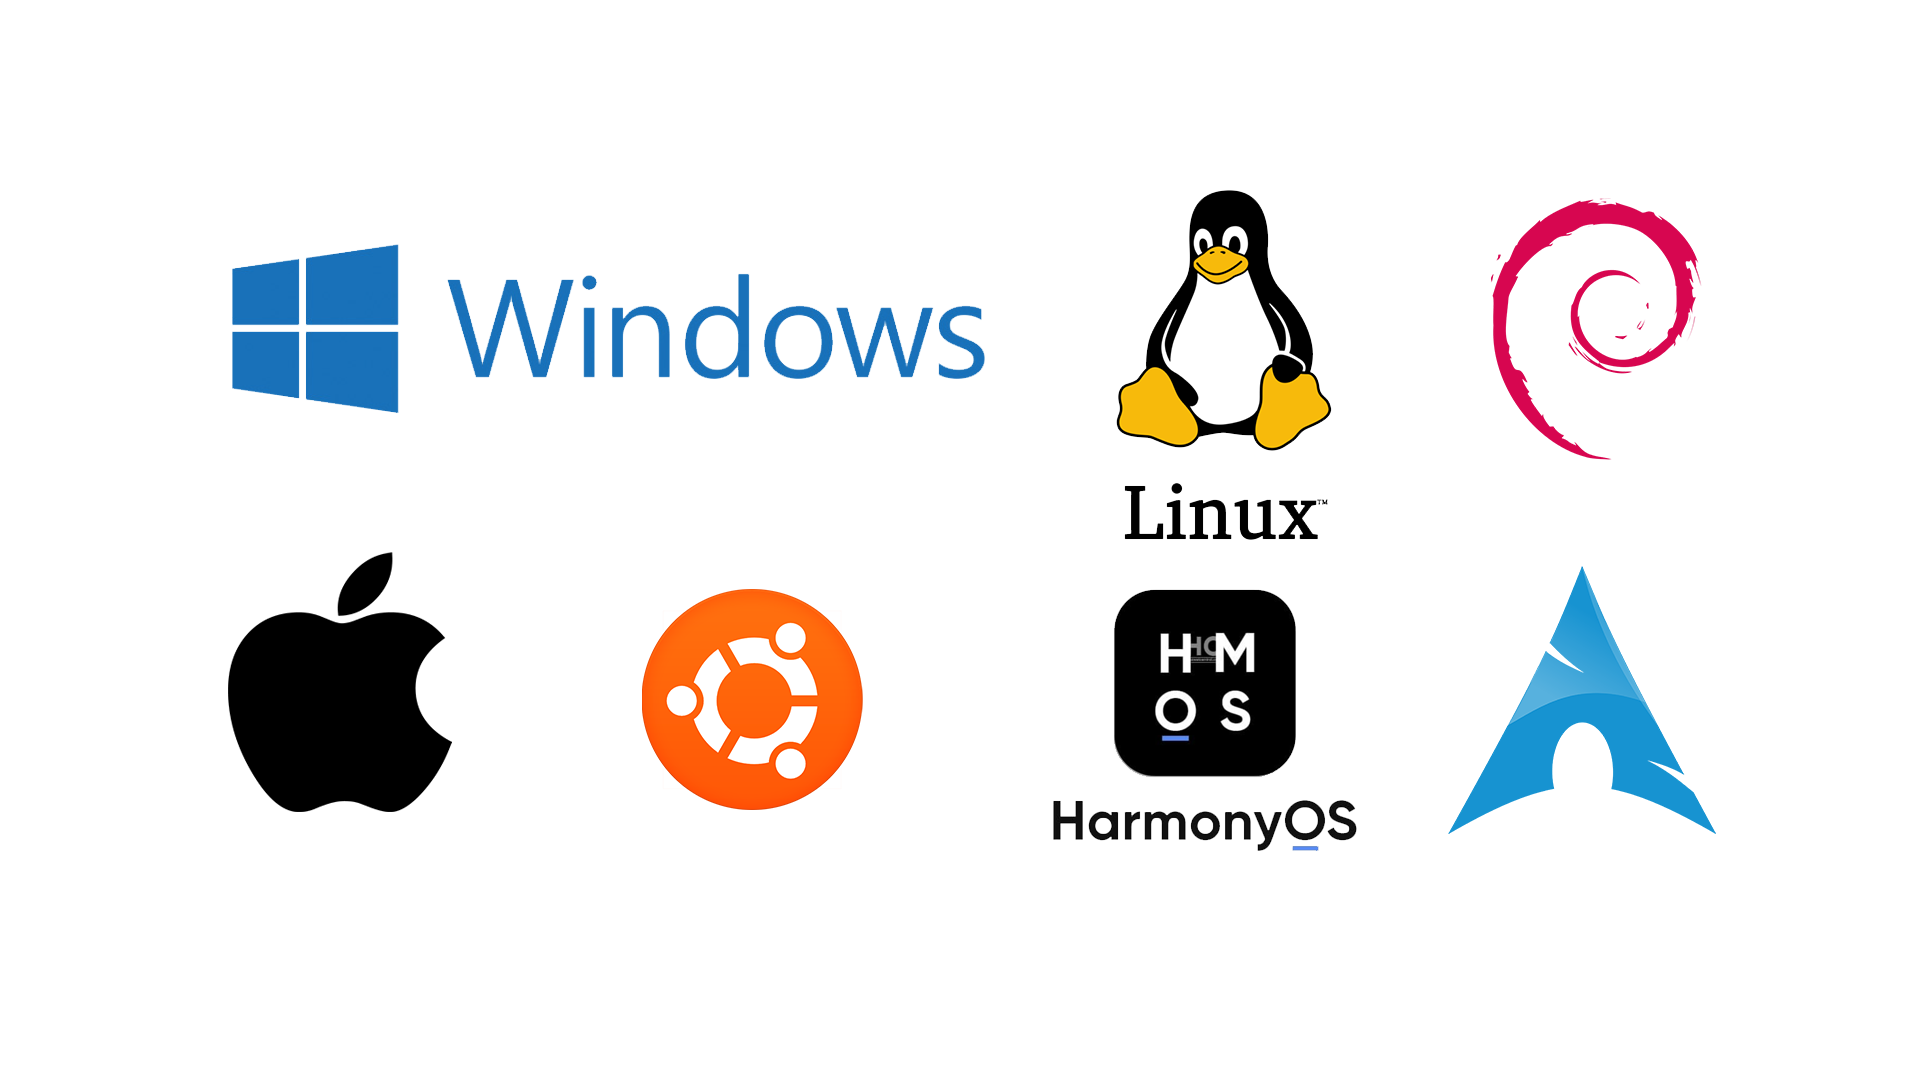
\includegraphics[width=0.8\textwidth]{day3/img/123.png}
			\end{figure}
		\end{column}
		\begin{column}{0.4\textwidth}
			\begin{minipage}[c][.5\textheight][c]{\linewidth}
				\begin{itemize}
					\item Windows\onslide<2>{:\textbf{ NT}}
					\item macOS, iOS\onslide<2>{:\textbf{ Darwin}}
					\item Linux, Android\onslide<2>{:\textbf{ Linux}}
				\end{itemize}
			\end{minipage}
		\end{column}
	\end{columns}
	\onslide<3>{
		\emoji{star} Operating System is \textbf{resource abstractor and resource allocator}.
	}
\end{frame}

\begin{frame}[fragile]{10k meter view of kernel code}
	\begin{columns}[T]
		\begin{column}{0.75\textwidth}
			\begin{minted}[fontsize=\small]{c}
void processEvent(event) {
    switch (event.type) {
        case NETWORK_COMMUNICATION:
            NetworkManager.handleEvent(event);
            break;
        case SEGMENTATION_FAULT:
        case INVALID_MODE:
            ProcessManager.handleEvent(event);
            break;
        // ...
    }
}
        \end{minted}
		\end{column}
		\begin{column}{0.2\textwidth}
			\begin{minipage}[c][.6\textheight][c]{\linewidth}
				\begin{itemize}
					\item \textbf{Event}
					\item \textbf{Handler}
				\end{itemize}
			\end{minipage}
		\end{column}
	\end{columns}
\end{frame}

\subsection{OS Events}


\begin{frame}[fragile]{OS Events}

	There are two kinds of events, we call them \textbf{Traps} in RISC-V\footnotemark:

	\begin{itemize}
		\item \textbf{Interrupts}: external asynchronous events
		      \begin{itemize}
			      \item Hardware-generated
			      \item e.g., some device controller says “something happened”
		      \end{itemize}
		\item \textbf{Exceptions}: unusual condition occurring at instruction run time
		      \begin{itemize}
			      \item Software-generated
			      \item e.g. a division by zero
		      \end{itemize}
	\end{itemize}

	\footnotetext{\href{https://zju-arch.pages.zjusct.io/arch-sp25/spec/riscv-unprivileged.html\#trap-defn}{1.6. Exceptions, Traps, and Interrupts}, RISC-V Unprivileged ISA Specification}

\end{frame}

\begin{frame}[fragile]{Trapped Control Flow}
	When a trap occurs, the control flow is switched to its handler:
	\begin{columns}
		\begin{column}{0.6\textwidth}
			\begin{figure}[H]
				\centering
				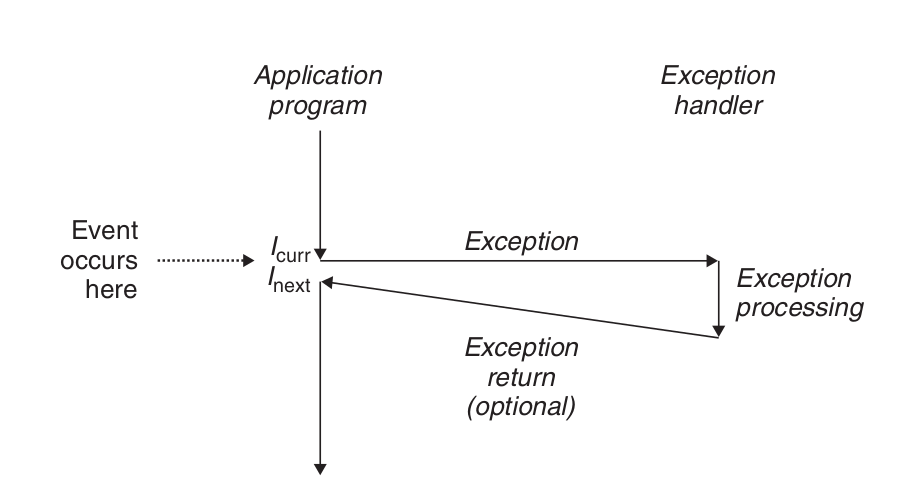
\includegraphics[width=\textwidth]{day3/img/interrupt-flow.png}
			\end{figure}
		\end{column}
		\begin{column}{0.4\textwidth}
			\only<1-2>{
				\begin{figure}[H]
					\centering
					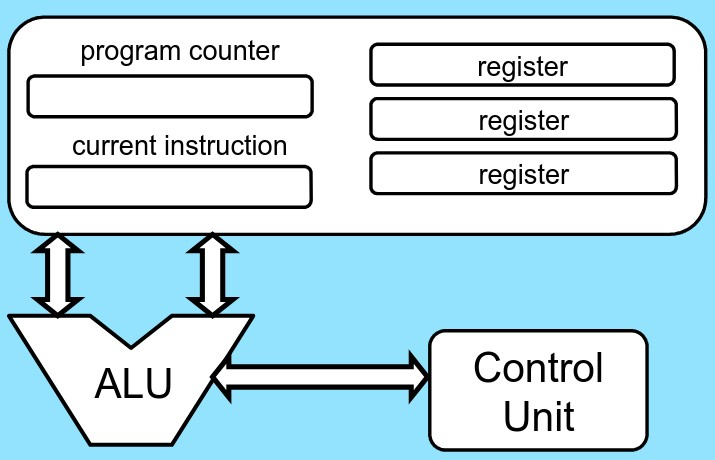
\includegraphics[width=\textwidth]{day3/img/cpu-abstract.jpg}
				\end{figure}
			}
			\only<3>{
				\begin{figure}[H]
					\centering
					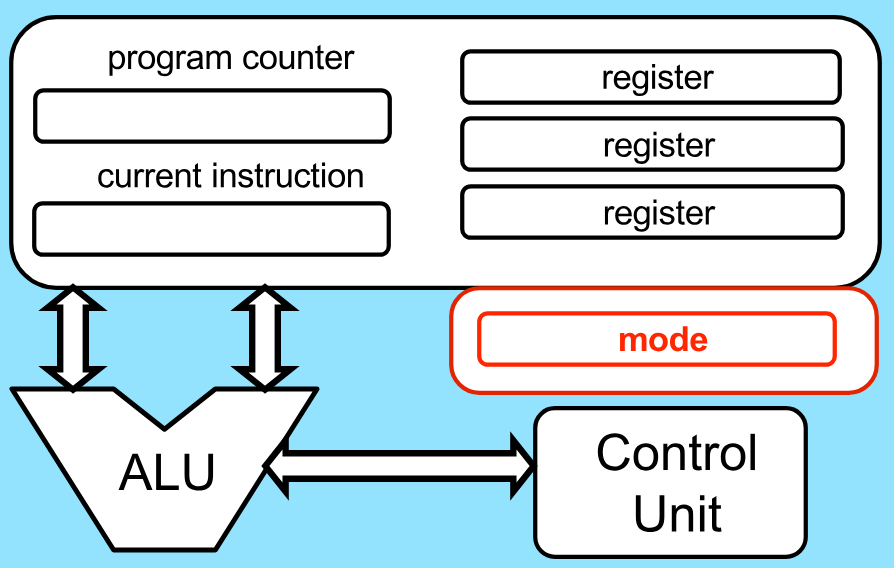
\includegraphics[width=\textwidth]{day3/img/mode-bit.png}
				\end{figure}
			}
		\end{column}
	\end{columns}
	\onslide<2->{\emoji{thinking} \textbf{Q: What do we need to separate the user and kernel space?}}

	\onslide<3>{\emoji{smirk} A: Add a \textbf{Mode Bit} to keep track of the current \textbf{privilege level}.}
\end{frame}

